\documentclass{article}

% Environment setup

\usepackage[
    margin=1.25in
]{geometry} %geometry (sets margin) and other useful packages 
\setlength{\oddsidemargin}{.25in}
\setlength{\evensidemargin}{.25in}
\setlength{\textwidth}{6in}
\setlength{\topmargin}{-0.4in}
\setlength{\textheight}{8.5in}
\setlength{\parindent}{0em}
\setlength{\parskip}{1em}

\usepackage{graphicx}
\usepackage{fancyref}
\usepackage[labelfont=bf]{caption}
\usepackage{subcaption}


\title{\textbf{CS 4641:} Supervised Learning}
\author{Bradley Reardon}
\date{February 10, 2019}

\begin{document}
    \maketitle

    \section{Introduction}
    The purpose of this assignment is to evaluate various supervised learning techniques in the context of two classification problems. We will focus on analyzing and adjusting five learning algorithms using two publically-available data sets, through cross-validation and hyperparameter adjustments. Then, we can use our adjusted models to compare supervised learning techniques in the context of each of our classification problems.

    \section{Classification problems}
    For the purposes of this report, data sets were obtained from the UCI Machine Learning Repository. Each data set downloaded was processed with a custom script in the corresponding folder, \textbf{process.py}, which randomly separated the data into an 80\% training data and 20\% test data split using the \textbf{train\_test\_split} function from scikit-learn. The split data was then serialized using Python's \textbf{pickle} module, to ensure that the training and test sets remained constant for evaluation.

    For the purposes of this assignment, cross-validation scoring of the various algorithms for each classification problem will be shown as the average score of 5-fold cross validation.

    \subsection{Car data set}
    The Car Evaluation Database was created in June, 1997 by Marko Bohanec. It contains 1728 instances and six attributes. The purpose of this database is to attempt to classify a car as an unacceptable, acceptable, good, or very good choice based on factors including cost of ownership, comfort, and safety. Full details about the data set can be found at the source link below.

    Note that this specific data set contains only categorical attributes. As scikit-learn does not support non-continuous variables, a one-hot encoder was used to re-encode categorical features into multiple dimensions.

    The problem at hand for this dataset is determining the acceptability for a car purchase based on the aforementioned attributes. Because this dataset notes that the instances in the data set completely cover the attribute space, this data set is interesting in particular due to its usefulness in comparing the optimization of different supervised learning algorithms.

    \textbf{Source:} https://archive.ics.uci.edu/ml/datasets/car+evaluation

    \subsection{Breast Cancer Wisconsin data set}
    The Breast Cancer Wisconsin data set was donated to the UCI Machine Learning Repository in 1992, and contains data from one doctor's clinical cases, gathered from January 1989 to November 1991. In total, there are 699 instances signifying information about breast tumors such as clump thickness, uniformity in shape and size, and other screening factors. Data points are identified by two classes -- benign or malignant. The features of the data points are encoded as 9 continuous attributes rating the screening factor from 1 to 10.

    This data set contains unknowns in the form of question marks in the data. To deal with this, missing values were imputed, calculating missing data points based on the mean of other points in the specific column of the missing attribute. 

    The problem at hand for this dataset is determining whether a tumor is benign or malignant based on tumor screening characteristics identified in the data set.

    \textbf{Source:} https://archive.ics.uci.edu/ml/datasets/Breast+Cancer+Wisconsin+\%28Original\%29

    \section{Decision trees with pruning}

    \subsection{Parameter selection}
    GINI criterion was selected because -- no discernible difference in training results, GINI is computationally faster

    Max depth, min samples per leaf methodology... Car seemed to have much lower accuracy with lower depth -- perhaps because the data set was complete. Chose max depth of 9 as a result. Cancer responsed better to more aggressive pruning with a max 

    \subsection{Performance}
    Wall clock time (pruning vs. nopruning)

    Learning curves for the car and breast cancer data sets, with and without pruning enabled, can be found in ~\Fref{fig:dt-learning}.

    \begin{figure}[htb]
    \centering

    \begin{subfigure}{0.5\textwidth}
      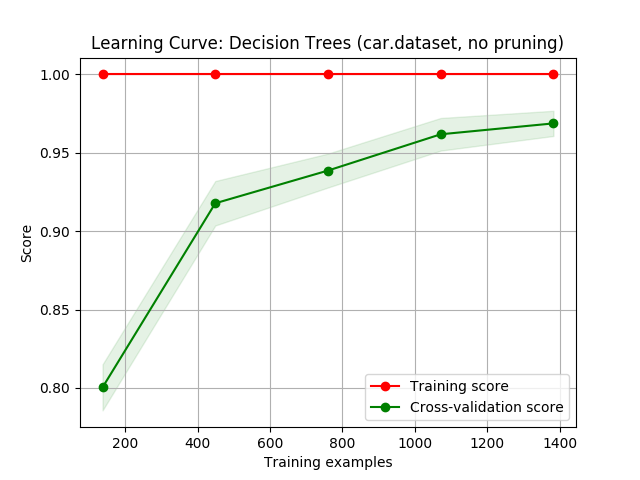
\includegraphics[width=\linewidth]{out/decision_tree_pruning/car-noprune-learning.png}
      \caption{Car data set, no pruning}
      \label{fig:dt-learning-1}
    \end{subfigure}\hfil
    \begin{subfigure}{0.5\textwidth}
      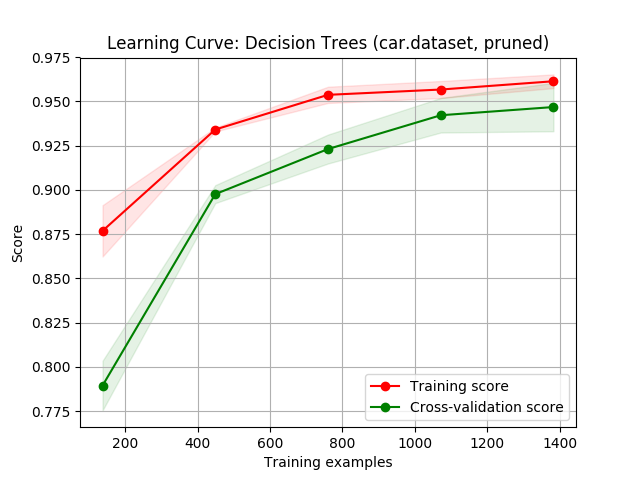
\includegraphics[width=\linewidth]{out/decision_tree_pruning/car-prune-learning.png}
      \caption{Car data set, with pruning}
      \label{fig:dt-learning-2}
    \end{subfigure}

    \medskip

    \begin{subfigure}{0.5\textwidth}
      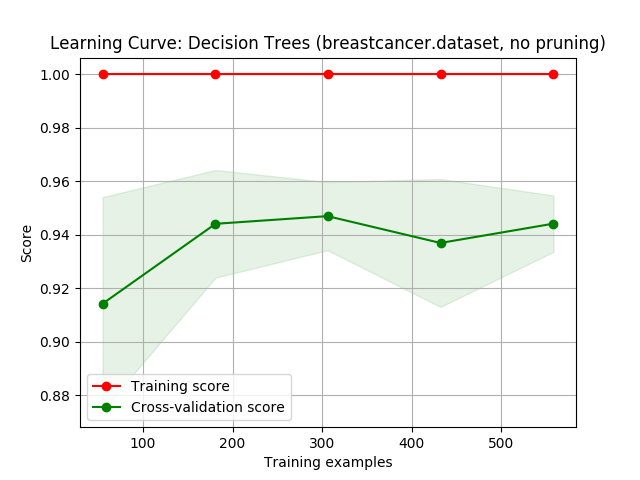
\includegraphics[width=\linewidth]{out/decision_tree_pruning/breastcancer-noprune-learning.png}
      \caption{Breast cancer data set, no pruning}
      \label{fig:dt-learning-3}
    \end{subfigure}\hfil
    \begin{subfigure}{0.5\textwidth}
      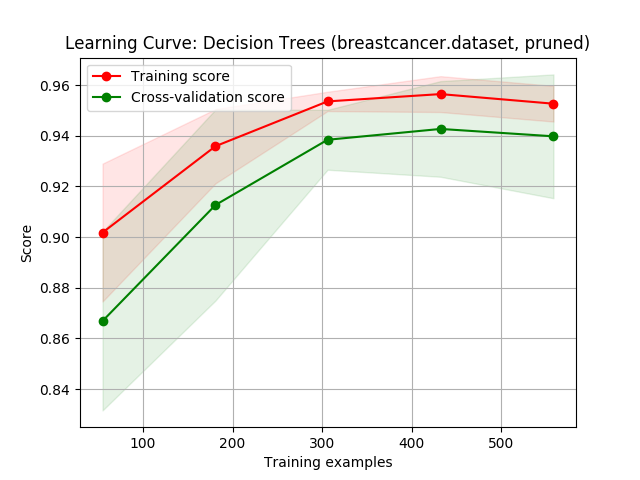
\includegraphics[width=\linewidth]{out/decision_tree_pruning/breastcancer-prune-learning.png}
      \caption{Breast cancer data set, with pruning}
      \label{fig:dt-learning-4}
    \end{subfigure}

    \caption{Learning curves for the car and breast cancer data sets using a decision tree classifier, with and without pruning.}
    \label{fig:dt-learning}
    \end{figure}


    \section{Neural networks}
    TODO

    \section{Boosting}
    TODO

    \section{Support vector machines}
    

    \subsection{Performance}

    Learning curves for the car and breast cancer data sets can be found in ~\Fref{fig:svm-learning}.

    \begin{figure}[htb]
    \centering

    \begin{subfigure}{0.33\textwidth}
      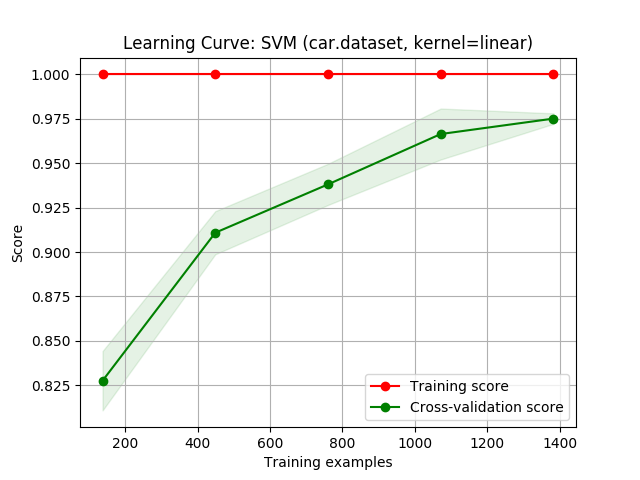
\includegraphics[width=\linewidth]{out/svm/car-kernel-linear.png}
      \caption{Car data, linear kernel}
      \label{fig:svm-learning-1}
    \end{subfigure}\hfil
    \begin{subfigure}{0.33\textwidth}
      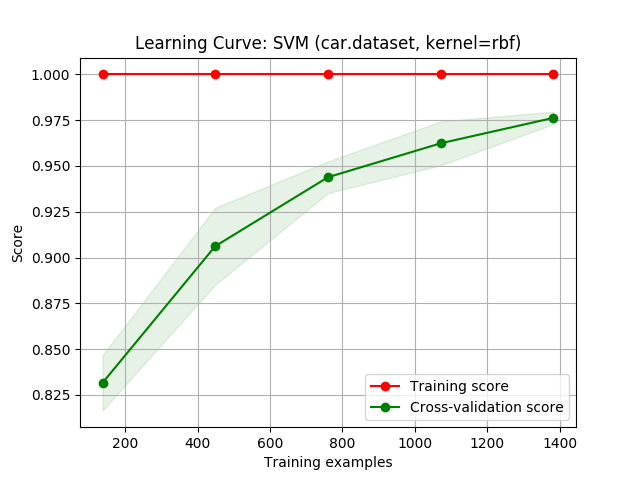
\includegraphics[width=\linewidth]{out/svm/car-kernel-rbf.png}
      \caption{Car data, RBF kernel}
      \label{fig:svm-learning-2}
    \end{subfigure}\hfil
    \begin{subfigure}{0.33\textwidth}
      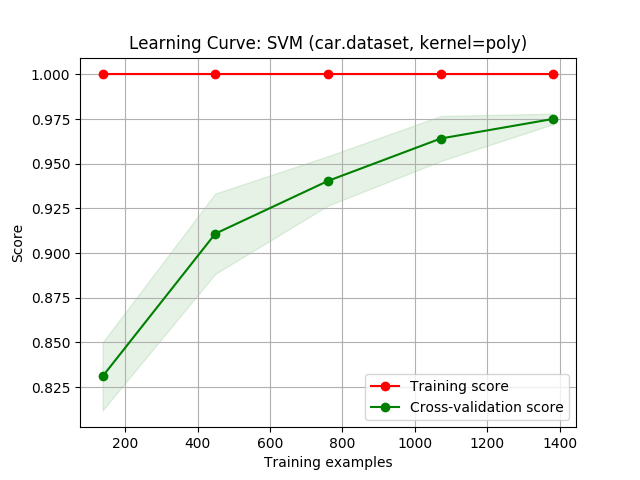
\includegraphics[width=\linewidth]{out/svm/car-kernel-poly.png}
      \caption{Car data, poly kernel}
      \label{fig:svm-learning-3}
    \end{subfigure}

    \medskip

    \begin{subfigure}{0.33\textwidth}
      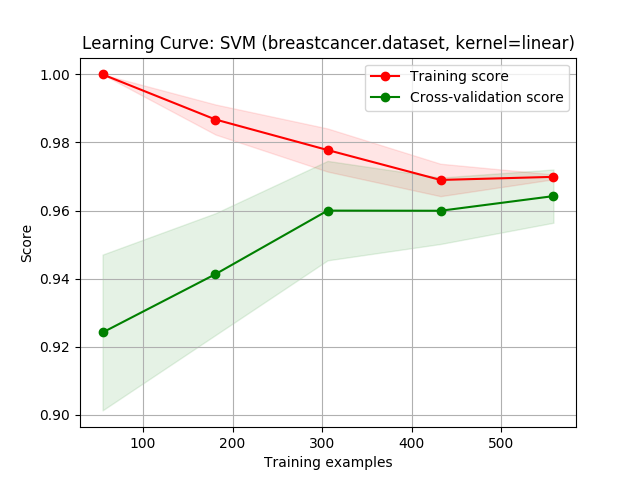
\includegraphics[width=\linewidth]{out/svm/breastcancer-kernel-linear.png}
      \caption{Breast cancer, linear kernel}
      \label{fig:svm-learning-4}
    \end{subfigure}\hfil
    \begin{subfigure}{0.33\textwidth}
      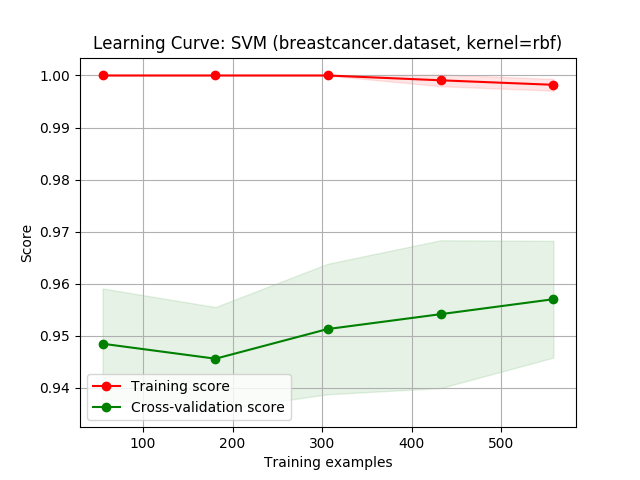
\includegraphics[width=\linewidth]{out/svm/breastcancer-kernel-rbf.png}
      \caption{Breast cancer, RBF kernel}
      \label{fig:svm-learning-5}
    \end{subfigure}\hfil
    \begin{subfigure}{0.33\textwidth}
      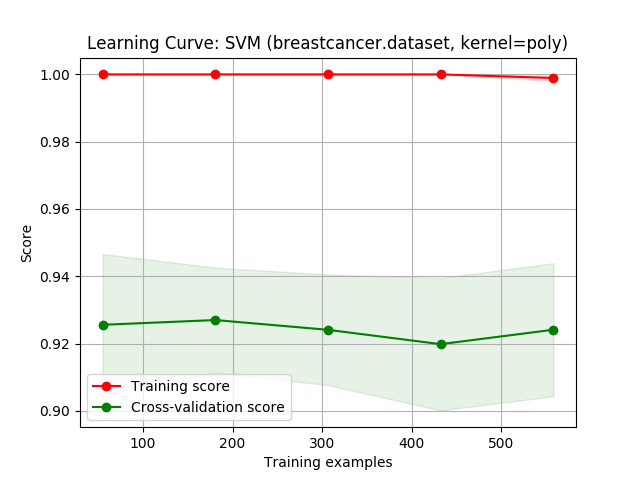
\includegraphics[width=\linewidth]{out/svm/breastcancer-kernel-poly.png}
      \caption{Breast cancer, poly kernel}
      \label{fig:svm-learning-6}
    \end{subfigure}

    \caption{Learning curves for the car and breast cancer data sets using an SVM classifier, with linear, RBF, and poly kernels.}
    \label{fig:svm-learning}
    \end{figure}

    \section{$k$-nearest neighbors}
    TODO

    \subsection{Parameter selection}
    car k=11
    cancer k=5

    Lowest k with highest cross-validation

    TODO ~\Fref{fig:knn-param}

    \begin{figure}[htb]
    \centering

    \begin{subfigure}{0.5\textwidth}
      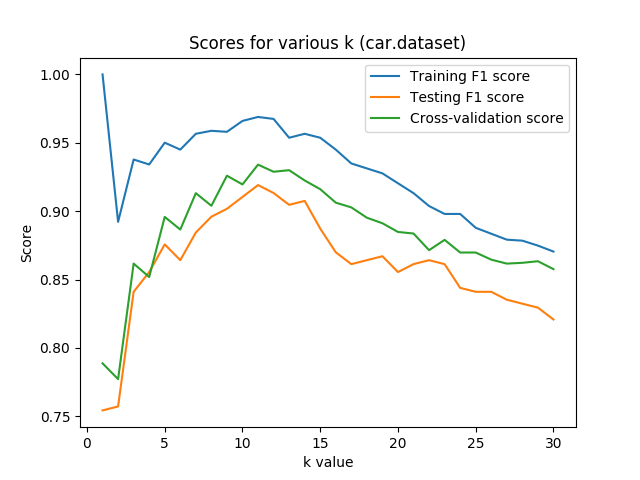
\includegraphics[width=\linewidth]{out/knn/car-k-testing.png}
      \caption{Car data set}
      \label{fig:knn-param-1}
    \end{subfigure}\hfil
    \begin{subfigure}{0.5\textwidth}
      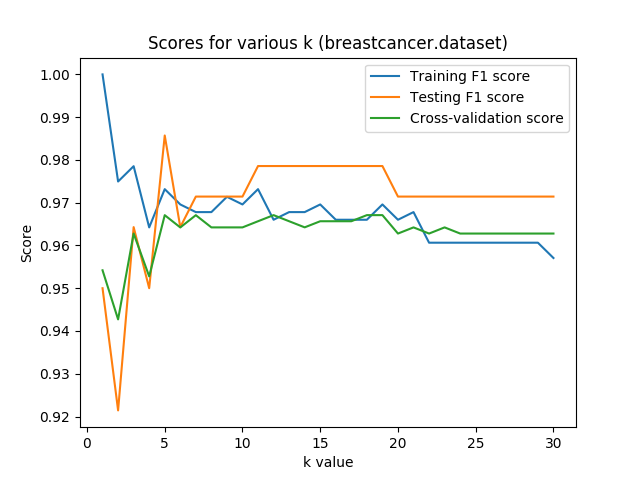
\includegraphics[width=\linewidth]{out/knn/breastcancer-k-testing.png}
      \caption{Breast cancer data set}
      \label{fig:knn-param-2}
    \end{subfigure}

    \caption{Testing $k$-nearest neighbors with various values of $k$}
    \label{fig:knn-param}
    \end{figure}

    \subsection{Performance}

    TODO ~\Fref{fig:knn-learning}

    \begin{figure}[htb]
    \centering

    \begin{subfigure}{0.5\textwidth}
      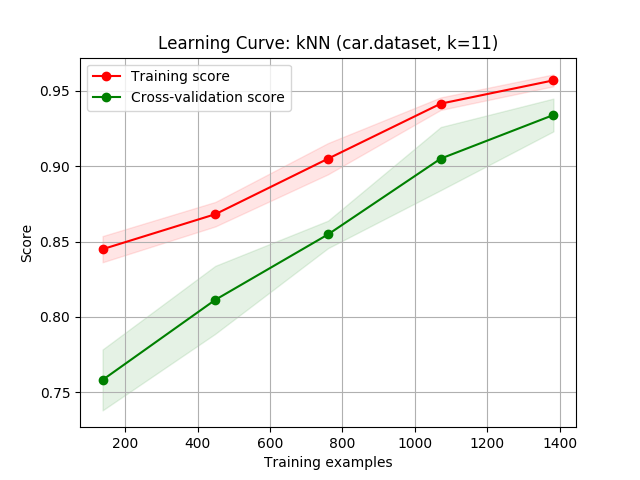
\includegraphics[width=\linewidth]{out/knn/car-k-11.png}
      \caption{Car data set, $k=11$}
      \label{fig:knn-learning-1}
    \end{subfigure}\hfil
    \begin{subfigure}{0.5\textwidth}
      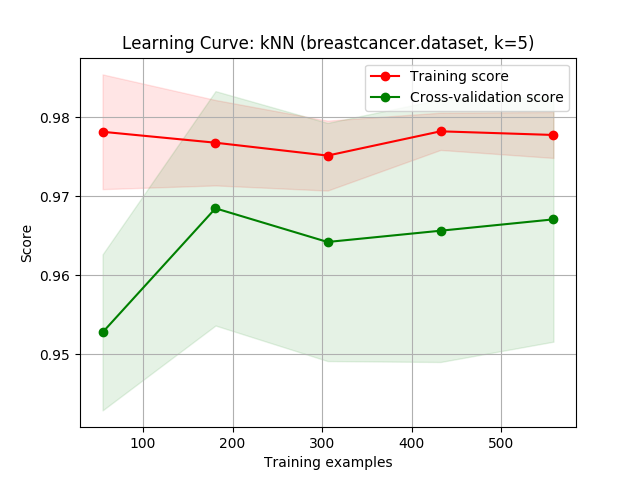
\includegraphics[width=\linewidth]{out/knn/breastcancer-k-5.png}
      \caption{Breast cancer data set, $k=5$}
      \label{fig:knn-learning-2}
    \end{subfigure}

    \caption{TODO TODO}
    \label{fig:knn-learning}
    \end{figure}

    \section{Analysis}
    TODO

    \section{Discussion}
    TODO

    \section{Conclusion}
    TODO
\end{document}